\chapter{مقدمه}
\label{chap:introduction}
تشخیص چهره یکی از روش‌های
\trans{احراز هویت بیومتریک}{biometric authentication}
است که در قدیم توسط سیستم‌های امنیتی پیشرفته انجام می‌شد. در روش‌های بیومتریک از اثر انگشت یا کل دست، عنبیه چشم، صدا، چهره و غیره استفاده می‌شود که متداول‌ترین آن استفاده از چهره فرد است. امروزه با توجه به پیشرفت تکنولوژی و همه‌گیر شدن آن تشخیص چهره را در گوشی‌های هوشمند همراه می‌توان یافت.
\\
همه گیری این تکنولوژی باعث پیشرفت‌های فراوان آن نیز شده است و امروزه گوشی‌های همراه می‌توانند به سرعت و با دقت بالا تشخیص چهره را انجام دهند و تقریبا به بهترین شکل اینکار را انجام می‌دهند. اما به امنیت این سیستم‌ها به اندازه کافی توجه نشده‌است. به این سیستم‌ها حملات متعددی صورت می‌گیرد که می‌توانند باعث خرابی سیستم، جعل هویت و یا گرفتن دسترسی کامل توسط حمله کننده و هکر شود. این سیستم‌ها به طور عمده امروزه بر اساس
\trans{شبکه‌های عصبی عمیق یا DNN}{Deep Neural Networks}
و
\trans{شبکه‌های عصبی کانولوشن یا CNN}{Convolutional Neural Network}
ساخته می‌شوند. در مقالات زیادی انواع حملات به این نوع شبکه‌ها بررسی شده‌اند.
\\
تشخیص حملات و مقابله با آن‌ها یکی از مواردی است که باید به آن توجه ویژه‌ای داشت. یکی از مشکلات اساسی در حملات و جعل تصاویر صورت گرفته دسته بندی حملات و تشخیص نوع حمله است که به آسانی توسط انسان امکان‌پذیر نیست.
\section{صورت مسئله}
تشخیص و دسته‌بندی حملات به سیستم‌های تشخیص چهره و جعل‌ تصاویر چهره از بزرگ‌ترین معزلات توسعه دهندگان این سیستم‌هاست. تضمین امنیت سیستم برای جلوگیری از دور زدن سیستم، گرفتن دسترسی‌های بیشتر و یا احراز هویت به جای فرد دیگری توسط هکرها از مواردی است که  توسعه دهندگان باید مد نظر داشته باشند. با توجه به اینکه به طور عمده حملات در دسته‌های مشخصی قرار می‌گیرند و ویژگی‌هایی دارند که می‌توان آن‌ها را دسته‌بندی کرد استفاده از روش‌های دسته‌بندی به شیوه‌های مختلف می‌تواند کارآمد و کمک‌کننده باشد.
\\
برای دسته‌بندی باید بتوانیم ویژگی‌های حملات مختلف را تشخیص دهیم. تشخیص این ویژگی‌ها به سادگی تشخیص ویژگی‌های تصاویر حیوانات مختلف برای دسته‌بندی آن‌ها نیست و ویژگی‌ها پیچیده‌تر و نیازمند سیستم‌های تشخیص دقیق‌تری هستند. بعد از تشخیص ویژگی‌های مورد نظر می‌توان حمله را دسته‌بندی کرد و متناسب با نوع حمله با آن مقابله کرد.

\section{اهداف پژوهش}
تجربه نشان داده است که یادگیری بدون نمونه برای دسته‌بندی و تشخیص نمونه‌هایی که کمتر تا کنون دیده شده‌اند یا اصلا دیده نشده‌اند، موفق عمل کرده و توانسته دسته‌بندی را به نحو احسنت انجام دهد. استفاده از یادگیری بدون نمونه در مواردی که پیدا کردن ویژگی‌های مشترک مانند حیوانات و اشیاء پیرامون به سادگی نیست و نمی‌توان فهرستی از ویژگی‌های مشترک را به آسانی تهیه کرد؛ موفق عمل کرده است. هدف پژوهش استفاده از دادگان‌های موجود و پر کاربرد در حوزه جعل تصویر چهره و یادگیری بدون نمونه برای ارائه راهکاری که قابلیت تشخیص و دسته‌بندی حملات مختلف به سیستم‌های تشخیص چهره را با دقتی نزدیک به دقت تشخیص چهره دارد، است.

\section{نوآوری پژوهش}
\section{ساختار پایان‌نامه}
در فصل دوم، به بررسی اجمالی درباره یادگیری بدون نمونه و انواع آن  می‌پردازیم و همچنین حملات و جعل‌های مختلف تصویر چهره را بررسی می‌کنیم. در فصل سوم، کارهای مرتبط به این پژوهش بررسی می‌شوند و مزایا و معایب آن‌ها به طور مختصر بررسی میگردد. در فصل چهارم، به تفضیل روش پیشنهادی و ایده اصلی بیان شده است. نحوه پیاده‌سازی و ساختار مدل بررسی شده‌است. در فصل ششم نتایج و ارزیابی‌های مرتبط بررسی شده و میزان کارایی و نتایج به‌دست آمده مورد تحلیل قرار گرفته‌است و در نهایت در فصل هفتم جمع‌بندی پایانی صورت گرفته‌است.
%
%روشی است که به طور معمول استفاده می‌شود. ماشین تعداد زیادی دادگان را ببیند و بر اساس آن‌ها تصمیم گیری کند که همانظور که گفته شد فرآیند یادگیری، فرآیندی طولانی است و نیازمند سیستم‌هایی قوی از لحاظ  سخت‌افزاری می‌باشد.
%
%روش بهبود یافته‌تر،
%\trans{یادگیری با چند نمونه}{few-shot learning}
%است که سعی بر این بوده تا مدل بر اساس دادگان محدودی یادگیری را انجام بدهد. برای کاهش وابستگی به داده روش
%\trans{یادگیری با یک نمونه}{one-shot learning}
%معرفی شد. در این روش ماشین برای تشخیص و دسته‌بندی یک داده جدید نیاز دارد تا یک نمونه از آن را حداقل از قبل دیده‌باشد و بر اساس آن فرآیند تشخیص را انجام دهد؛ برای مثال: در متون نوشته شده برای تشخیص زبان استفاده شده می‌تواند کاربردی باشد.
%\cite{Koch}
%در آخر روش
%\trans{یادگیری بدون نمونه}{zero-shot learning}
%مطرح شده است. هدف این روش این است که ماشین بدون اینکه یک نمونه جدید را از قبل دیده باشد بتواند آن را دسته‌بندی کند و تشخیص دهد. به طور مثال می‌تواند در تشخیص گونه‌های جدید جانوری یا گیاهی کاربرد داشته باشد.
%
%\section{یادگیری مادام‌العمر}
%فرآیند یادگیری می‌تواند مادام‌العمر ادامه پیدا کند و مدل روز به روز بهبود پیدا کند به طور مثال در فرآیند تشخیص ژست و نوع حرکات انسان همواره حرکات جدیدی را می‌توان داشت که با حرکات قبلی متفاوت هستند. دسته‌بندی این حرکات و درک مفهوم آن‌ها می‌تواند به ما کمک کند تا در کاربرد‌هایی مانند: تشخیص بیماری‌ اوتیسم، درک و ترجمه زبان ناشنوایان و تشخیص ناهنجاری‌های حرکتی بتوانیم بهتر عمل کنیم.
%ویدیوی
%\cite{L2L}
%در یوتیوب کاربرد یادگیری بدون نمونه را در تشخیص ژست و نوع حرکات دست استفاده کرده است.(شکل
%\ref{report:gesture}
%) چگونگی تشخیص نوع حرکات دست، زاویه چرخش، رو و پشت بودن دست، جهت حرکت دست و ویژگی‌هایی از این قبیل را بررسی کرده است.
%
%\begin{figure}[h]
%	\centering
%	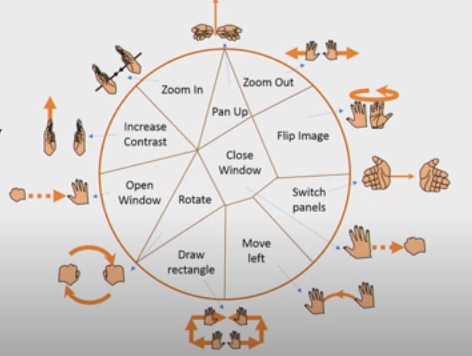
\includegraphics[width=0.6\textwidth]{img/report/gesture}
%	\caption{تشخیص ژست \cite{L2L}}
%	\label{report:gesture}
%	\centering
%\end{figure}
%
%\section{فرا یادگیری}
%روش
%\trans{فرا یادگیری }{meta learning}
%در چند سال اخیر مطرح شده است. در ادامه فرآیند بهینه سازی روش‌های یادگیری در این روش هدف
%\trans{ یادگیری مسیر یادگیری}{learn the learning process}
%است؛ یعنی، دنبال راهکاری باشیم که مسیر یادگیری را بتوانیم بهینه کنیم.\cite{metaLearning1}
%\cite{metaLearning2}
%تفاوت عمده انسان با ماشین‌ و روش‌های سنتی استفاده شده این است که انسان یاد می‌گیرد که چگونه یاد بگیرد. در روش‌های سنتی یادگیری ماشین داده‌ها به دو دسته آموزشی و آزمایشی تقسیم می‌شوند و با اجرای فرآیندی روی آن‌ها ماشین قادر به تشخیص خواهد بود و همواره این مسیر باید تکرار شود. این روش سعی دارد تا با بررسی فرآیند یادگیری، نحوه مقدار دهی اولیه شبکه، یادگیری پارامترهای متا و مواردی دیگر بتواند یادگیری ماشین را به یادگیری انسان نزدیک‌تر کند.
%
%\section{سخن پایانی}
%
%در رابطه با روش‌های یادگیری بدون نمونه و فرا یادگیری دو مخزن گیت‌هاب
%\cite{awesomeZeroShot}
%\cite{AwesomeMeta}
%که مقالات، پایگاه های داده و کد‌های مرتبط با مباحث بحث شده را جمع‌آوری کرده‌اند؛ جزو مراجع مناسب برای جمع آوری اطلاعات هستند و در این گزارش از آن‌ها استفاده شده‌است.
